% example tikz figure

\documentclass{article}

\usepackage{tikz}
\usetikzlibrary{arrows,shapes,positioning,shadows,trees}


\begin{document}

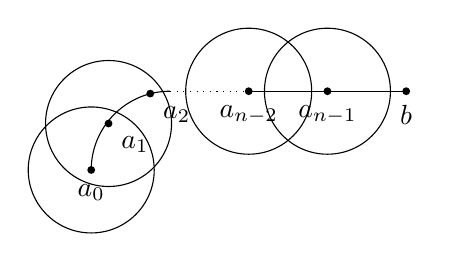
\begin{tikzpicture}
    % arc from (-1,0) to (0,0) with center (0, -1)
    \draw (-1,0) arc (180:90:1);
    % line from (0,0) to (3,0), with large dots
    \draw[dotted] (0,1) -- (1,1) ;
    % line from (1,1) to (3,1)
    \draw (1,1) -- (3,1);
    % mark (-1,0) as a_0 at the bottom, fill the node
    \node[fill,circle,inner sep=1pt,label=below:$a_0$] at (-1,0) {};
    % mark on the arc at x=-2/3 as a_1 at the bottom, fill the node
    \node[fill,circle,inner sep=1pt,label=below right:$a_1$] at (-0.78,0.59) {};
    % mark on the arc at x=-0.25 as a_2 at the bottom, fill the node
    \node[fill,circle,inner sep=1pt,label=below right:$a_2$] at (-0.25,0.97) {};

    % mark a_{n-2} at (1,1) at the bottom, fill the node
    \node[fill,circle,inner sep=1pt,label=below:$a_{n-2}$] at (1,1) {};
    % mark a_{n-1} at (2,1) at the bottom, fill the node
    \node[fill,circle,inner sep=1pt,label=below:$a_{n-1}$] at (2,1) {};
    % mark b at (3,1) at the bottom, fill the node
    \node[fill,circle,inner sep=1pt,label=below:$b$] at (3,1) {};

    % for every node mentioned above, draw a cricle with radius 1.5
    \draw (-1, 0) circle (0.8);
    \draw (-0.78, 0.59) circle (0.8);
    % \draw (-0.25, 0.97) circle (1);
    \draw (1, 1) circle (0.8);
    \draw (2, 1) circle (0.8);
\end{tikzpicture}
\end{document}